\section{Rational Proofs, Profit and Multiple Delegations}

\begin{frame}{From Reward to Profit}
		\begin{itemize}[<+- | alert@+>]

			\item In rational proofs ``honesty'' guarantees \textit{highest reward} $R^*$.
			\item \textbf{Observation:} The computation of a honest worker requires more effort than that of a negligent one.
			%		\item \textbf{NB:} We interpret "Cost" as the \# of gates the prover actually computed.
		\end{itemize}
		\pause	
		\bigskip
		
		\center{\large{\textbf{Q:} Does honesty in rational proofs also guarantee\\ \textit{highest \textbf{profit}}?}}
		\pause
		
		(Where the profit of a prover is $R-C$).
\end{frame}

\begin{frame}{Highest Profit is Guaranteed for a Single Honest Delegation) [AM13,GHRV15]}
	% So far we talked only about rewards, but we also want to talk about profits
	% Why? it's more realistic. It allows for example to ask if RPs are individually rational for the prover.

	\begin{itemize}[<+- | alert@+>]
		\item Consider a ``lazy'' prover $\tilde{P}$:
		\begin{itemize} 
			\item investing (somewhat small) effort $\tilde{C}$;
			\item receiving a (somewhat small) reward $\disR$. 
		\end{itemize}
		
		\item \textbf{The goal:} ``honest profit always larger than dishonest profit''. \onslide<+-> i.e.
		$$R^*-C^* \geq \tilde{R}-\tilde{C}$$
		\begin{itemize}
			\item sufficient that $R^* - \tilde{R} \geq C^*$
		\end{itemize}
		
		\item Consider the quantity $\Delta := min_{\tilde{P}}[R^*-\tilde{R}]$
		
		
		\item \textbf{Scaling suffices:} Scale the reward by a factor $C^*/\Delta$.
	\end{itemize}
	
	\onslide<+->
	\bigskip
	\noindent
	\large{\textbf{Can we apply the same solution if we delegate more than one problem?}}
\end{frame}


\begin{frame}{Profit and Multiple Inputs}
	%\textbf{An intuitive example: } SETI@home and gridcoin.
	% Why would the case for multiple inputs be different?
	%\pause
	\begin{itemize}[<+- | alert@+>]
		\item Assume I can solve \textit{correctly} a single input $x$ in time $T$.
		\item But I could (somewhat) incorrectly solve two inputs $x,x'$ at the same time.
	\end{itemize}
	\onslide<+->
	
	\textbf{Then we don't want (something like) this to happen:} \onslide<+->
	
	$ \textcolor{green}{y} \rightarrow \$\$\$ $ %\begin{flushright} (one correct output) \end{flushright}
	\onslide<+->
	
	but\\
	$ \textcolor{red}{y} + \textcolor{red}{y'} \rightarrow \$\$ + \$\$ $ %\begin{flushright} (two incorrect outputs) \end{flushright}
	\onslide<+->
	\begin{block}{We don't want, e.g., two incorrect outputs to generate more profit than a single correct one.}
		\pause \small{(Notice we assume \textit{costs and rewards are additive} among different inputs)}
	\end{block}
		\onslide<+->
		\medskip
		
		\alert{Unfortunately this is the case in some rational proofs.}
\end{frame}


\begin{frame}{``Bad Incentives'' with Multiple Inputs [\textbf{C}G15]}
	\large{\textbf{How much does a worker earn by just replying at random (a $O(1)$-cost strategy)?}}
	\pause
	\begin{columns}
		\column{0.60\textwidth}
		\begin{align*}
		\tilde{R} &=E_{m,b}[BSR(\frac{m}{n}, b)] \\
%		&= \frac{1}{n+1}\sum_{m=0}^{n} E_b[BSR(\frac{m}{n},b] \\
%		&= 
%		\frac{1}{n+1}\sum_{m=0}^{n}(2(2p \cdot \frac{m}{n}-\frac{m^2}{n^2}-p+1))
%		\\
		&=2-\frac{2n+1}{3n} > 1
		\end{align*}
		\pause
		Whereas for the honest prover:
		\[
		R^* \leq 2
		\]
		\column{0.40\textwidth}
		\onslide<1->
		\begin{figure}
			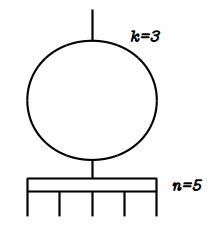
\includegraphics[scale=0.7]{pics/threshold-circ.png}
			
		\end{figure}
	\end{columns}
	\pause

	\noindent
\textbf{Conclusion:} Two random outputs are more profitable than a correct one.
\end{frame}


\begin{frame}{Definition of Sequential Composability}
		
		\begin{block}{Desired Guarantee:}
		A worker cannot gain more than $\epsilon$ from investing in several, incorrect computations instead of a single correct one.
		\end{block}
		
		\bigskip
		\pause
		
		\begin{framed}
		A rational proof $(P,V)$ for $f$ 
		is $\epsilon$-{\sf sequentially composable}\footnote<2->{some details of the definition are missing for clarity} for an input distribution $\cal D$, if:
		\begin{itemize}
			\item  for every prover $\disP$, 
			\item	$x,x_1,\ldots,x_k$ drawn according to ${\cal D}$,
		\end{itemize}
		 $$C(x) \geq \sum_{i=1}^k 
		\tilde{C}(x_i)\implies \sum_{i}\tilde{R}(x_i) - R \leq \epsilon$$
		\end{framed}
		
\end{frame}

\begin{frame}{A Sequentially Composable Protocol for Arithmetic Circuits [\textbf{C}G15]}
		\begin{block}{\large{Result}}
		\large{We build sequentially composable rational proofs for (a subset of) arithmetic circuits of $\log$-depth and $\poly$-size.} with:
		\begin{itemize}
			\item $\log n$ rounds;
			\item polylog communication;
			\item polylog verifier.
			\item $O(T)$ prover.
		\end{itemize}
		\end{block}
\end{frame}



